\section{Teilversuch 2: Messung des Elektronenstrom als Funktion der Anodenspannung für Neon}
	Die optimale Messkurve und die entsprechende Einstellungen finden Sie im Laborprotokoll. 

	\subsection{Zur Frage 2}
		$U_1$ ist die Spannung zwischen die Kathode und das Gitter $A1$, ist also die "Saugspannung". Sie besagt wie viel Elektronen im Stoßbereich ($A1 \cdots A2$) ausgelöst wird. Je höher die Anzahl der Elektronen, desto höher der Strom $I_A$ im Allgemein. Wegen der linearen Anstieg der Spannung $U_{B1}$, kann man die horizontale Achse auch als Zeit betrachten. Die Fläche unter die Kurve kann man somit als die Gesamtanzahl an Elektronen, die bei der Anode ankommen. Somit:
		\begin{align}
			\uparrow U_1 ~\Rightarrow~ \uparrow \text{ Anzahl }e^- ~\Rightarrow~ \uparrow \text{ Kurvesteigung}
		\end{align}
		Deswegen kann man durch erhöhen (bzw. verkleinern) der Spannung $U_1$ steuern, wie steil die Kurve ist. 

		\begin{wrapfigure}{r}{0.5\textwidth} 
		    \centering
		    \vspace{-2em}
		    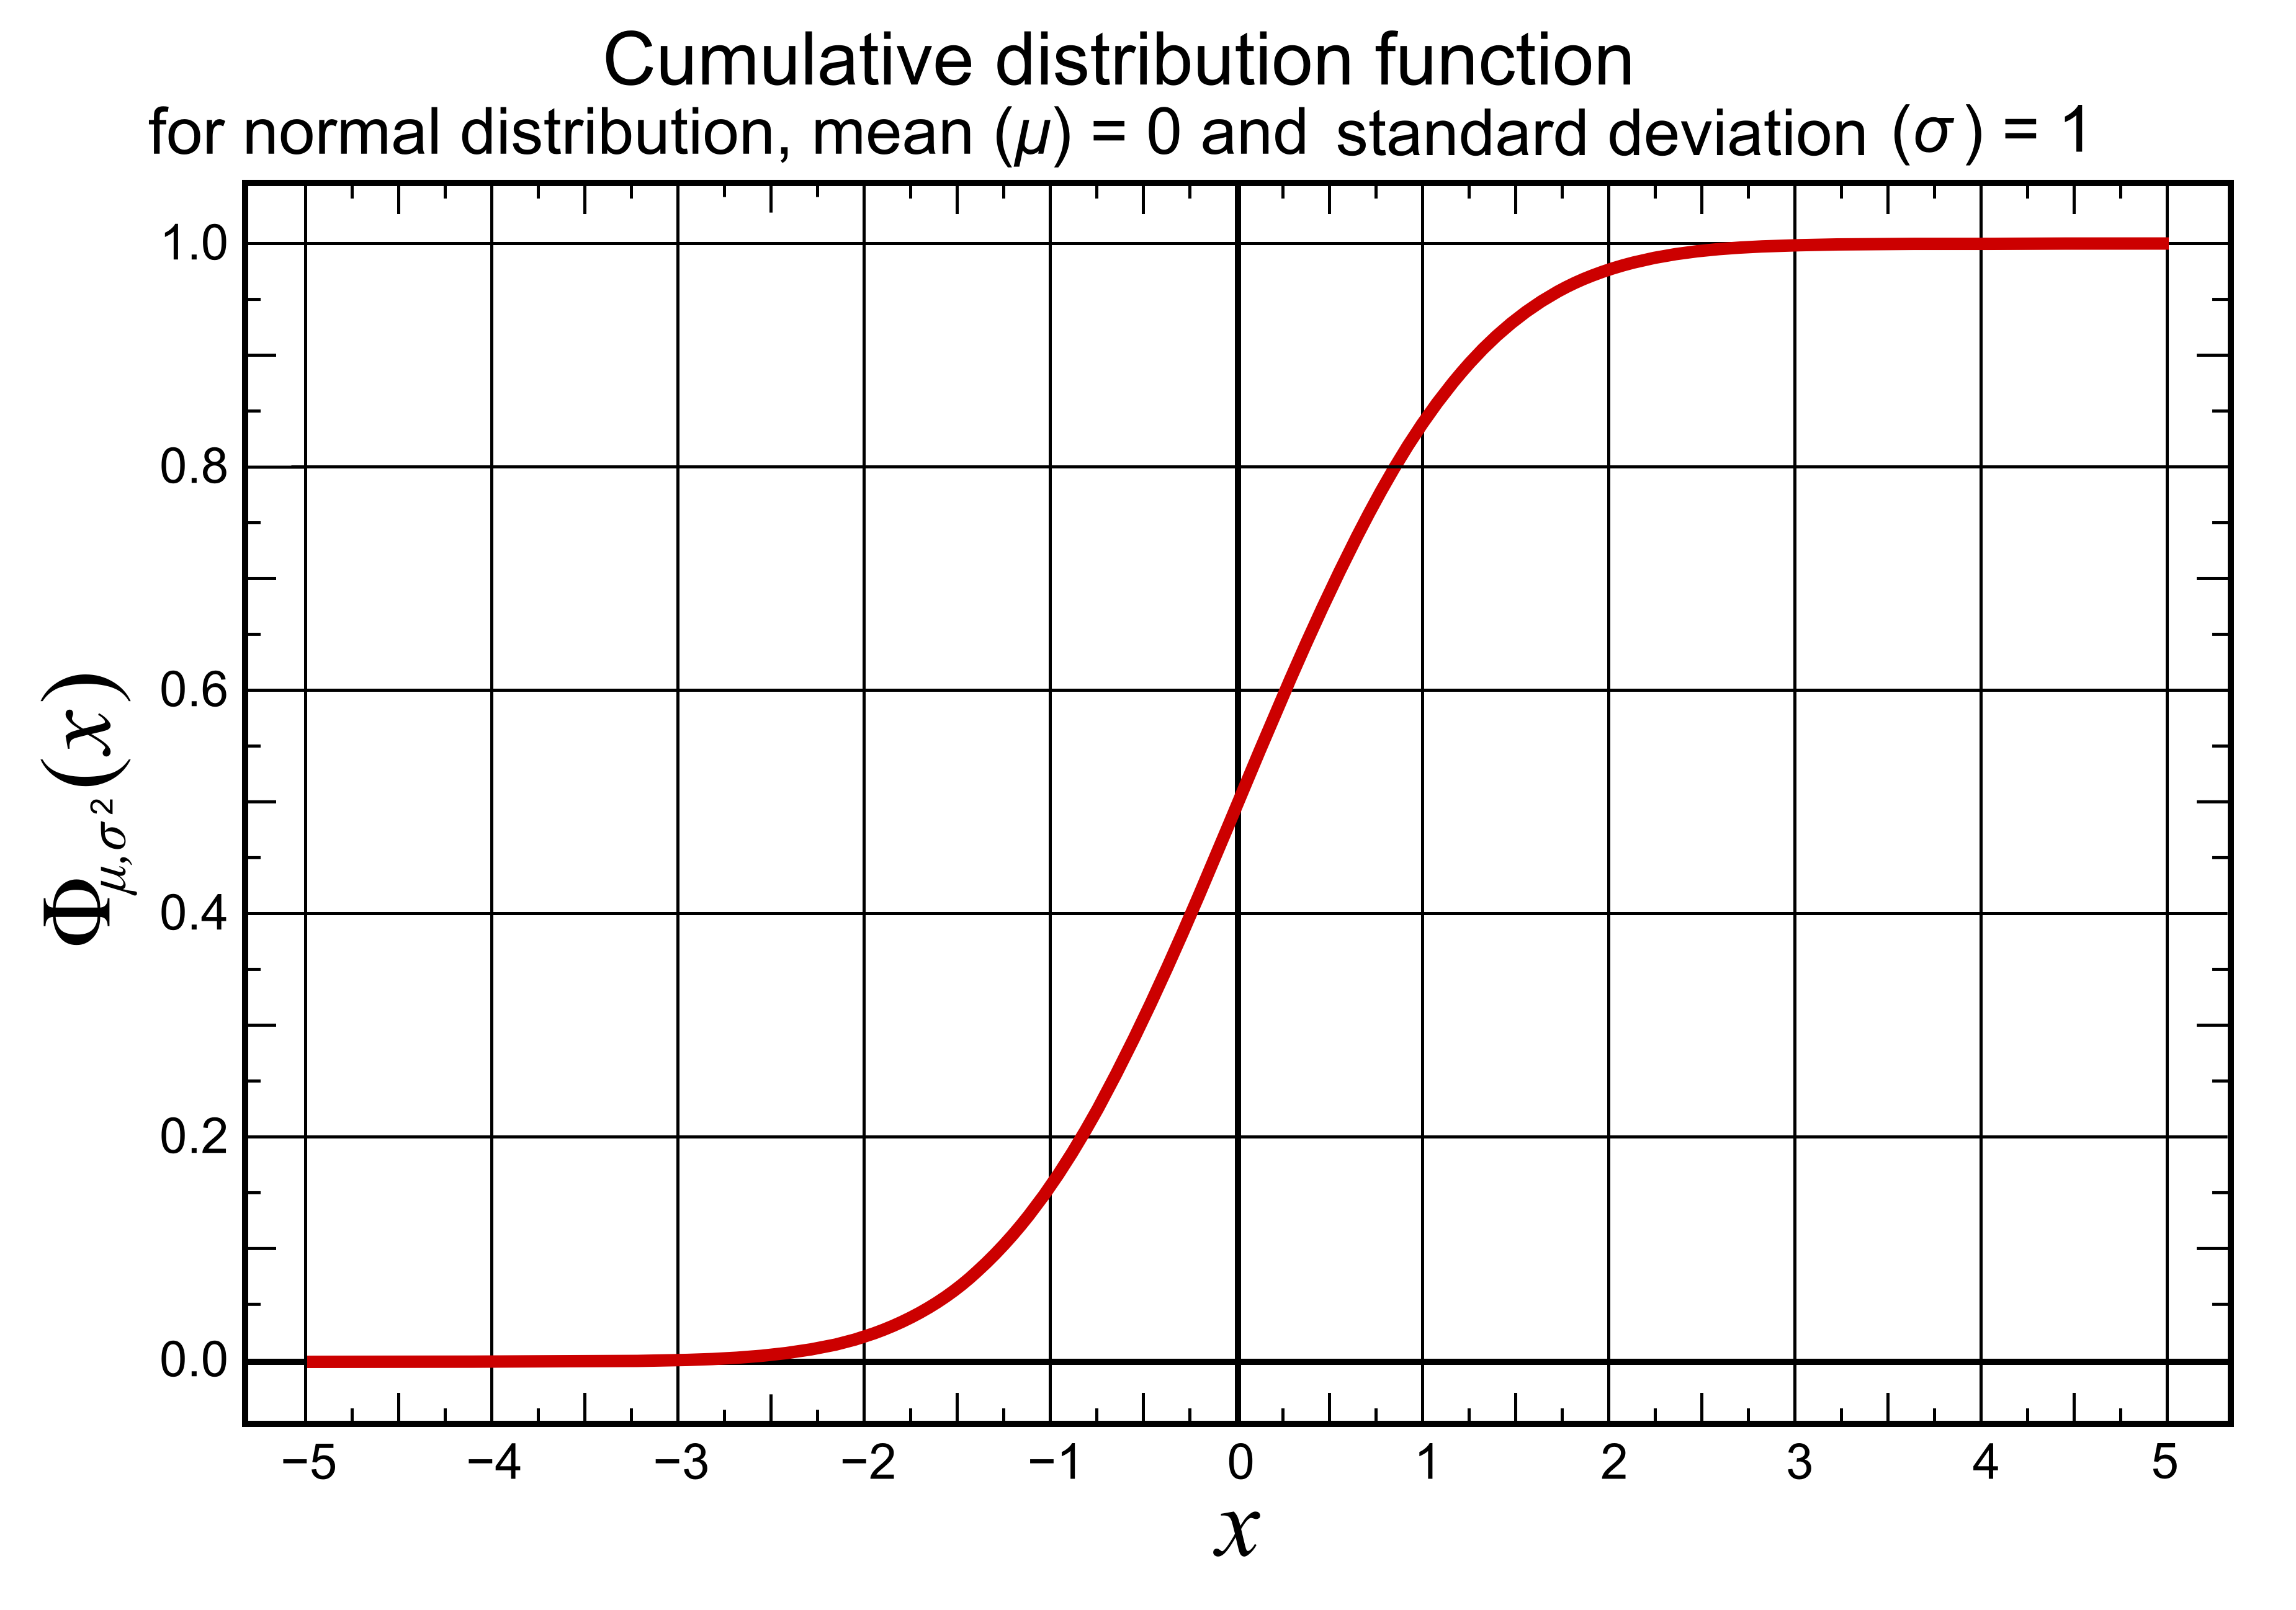
\includegraphics[width=0.5\textwidth]{images/gauss_cdf.png}
		    \vspace{-1em}
		    \caption{Gaußische kumulierte Verteilungsfunktion, \cczero{} Wikimedia \textit{User:Mikael\_Häggström}}
		    \vspace{-2em}
		    \label{fig:gauss-cdf}
		\end{wrapfigure}

		$U_3$ ist die Spannung zwischen das Gitter $A2$ und die Anode, ist also die "Gegenspannung". Sie ist mit der elektrischen Feld zwischen $A1$ und $A2$ entgegesetzt, und deswegen bremst die Elektronen, die durch das Gitter $A2$ durchkommt. Elektronen, die nicht genug Energie haben, um diese Gegenspannung $U_3$ zu überwinden, können somit die Anode nicht erreichen. Sie funktioniert somit als Energieschwelle. 

		Da die Stoße ein statistische Prozess ist, kann man ein gaußformige Verteilung der Elektronenergie vorstellen. Somit sieht die Anzahl der Elektronen, die die Anode erreichen, wie die Kurve in Abbildung \ref{fig:gauss-cdf}, wobei horizontale Achse die Spannung $U_3$ zugeordnet werden kann. Allerdings ist die Kurve gespiegelt: mit einer höheren Spannung $U_3$ gibt es weniger Elektronen und bei einer niedrigen Spannung $U_3$ mehr. 

		Da die Strom $I_A$ bei der Minima genau die Anzahl die Elektronen besagt, die bei einer bestimmten Beschleunigungsspannung $U_2$ durchkommen, kann man die Spannung $U_3$ erhöhen, um die Minimawerten zu reduzieren (oder auch umgekehrt). Dadurch kann man dann die Ausprägung von Minima und Maxima steuern. 

	\subsection{Zur Frage 3}
		Während des Anstiegs der Beschleunigungsspannung $U_2$ sieht man leuchtende Wolke/Schichten, die Richtung Gitter $A1$ bewegen. Ab eine bestimmte Punkt entsteht noch eine Wolke, was wiederum Richtung Gitter $A1$ bewegen. Am Ende gab es im Rohr 3 leuchtende Wolken. Siehe Laborprotokoll für die genauere Zeichnung. 

		Dazu kann man das Effekt in zwei Teile unterscheiden:
		\begin{enumerate}
			\item Das Leuchten \par
				Wenn es Elektronen gibt, welche Energie genau die Energieunterschied $\Delta E_{1 \rightarrow 2}$ entsprechen, dann werden \ce{Ne}-Atome nach einem Stoß angeregt. Da der angeregte Zustand nicht stabil ist, zerfällt das 
				Atom sofort und ein Photon wird dann durch spontane Emission gestrahlt. Diese Photonen sehen wir dann als Leuchten.
			\item Bewegung Richtung Gitter $A1$ \par
				Siehe Laborprotokoll für eine Zeichnung. Die Spannung $U_1$ regelt die E-Feldstärke entlang der $A1\cdots A2$ Achse. Je größer der E-Feldstärke, je kurzer die Strecke, die ein Elektron braucht, um auf die benötigte Energie zu beschleunigen. Somit schiebt sich der Punkt, wobei ein Elektron ein \ce{Ne}-Atom anregen kann, in Richtung Gitter $A1$, wenn $U_1$ erhöht ist. \par
				Wenn $U_1$ groß genug ist, kann Elektronen mehrmals in der Flugstrecke die benötigte Energie vom E-Feld gewinnen, somit entstehen mehrere leuchtende Wolken.
		\end{enumerate}

	\subsection{Zur Frage 4}
		Da es nur zwei Minima in der Graphik gibt, gibt es nur einen Abstand, den man für die Berechnung der Energieniveau verwenden kann. Wir schätzen nun der Fehler der Spannung bei den Minima als $\Delta U_{B1} = \SI{0.03}{\volt}$, da diese die Auflösung der Tabelle im Programm war. 

		Der Abstand $d$ zwischen der zwei Minima ist somit:
		\begin{align}
			d &= \SI{6.17}{\volt} - \SI{4.26}{\volt} = \SI{1.91}{\volt} \\
			\Delta d &= \addquad{\SI{0.03}{\volt}, \SI{0.03}{\volt}} = \SI{0.04243}{\volt} \sigfig{4}
		\end{align}
		Also erhalten wir mit $U_{B1} = U_2 / 10$: $d = \SI{19.1(5)}{\volt}$. Das entspricht ein Energieunterschied $\Delta E = \SI{19.1(5)}{\electronvolt}$, was ein Photon mit der Wellenlänge:
		\begin{align}
			\lambda &= \frac{hc}{E} = \SI{649.132}{\nano\meter} \sigfig{6} \\
			\Delta \lambda &= \abs{-\frac{hc}{E^2}\Delta E} = \SI{16.993}{\nano\meter} \sigfig{5}
		\end{align}
		oder $\lambda = \SI{649(17)}{\nano\meter}$.

		Aus dem NIST Datenbank \citep{NIST_ASD} für \texttt{[Ne I]} ($= \ce{Ne^{0+}}$) haben wir die folgende Emissionslinie zur Auswahl: 
		\begin{multicols}{4}
			\begin{itemize}
				\item \SI{632.81646}{\nano\meter}
				\item \SI{633.08894}{\nano\meter}
				\item \SI{633.44276}{\nano\meter}
				\item \SI{635.18532}{\nano\meter}
				\item \SI{636.49963}{\nano\meter}
				\item \SI{638.29914}{\nano\meter}
				\item \SI{640.1076}{\nano\meter}
				\item \SI{640.22480}{\nano\meter}
				\item \SI{640.97469}{\nano\meter}
				\item \SI{642.17044}{\nano\meter}
				\item \SI{644.47118}{\nano\meter}
				\item \SI{650.65277}{\nano\meter}
				\item \SI{653.28824}{\nano\meter}
				\item \SI{659.89528}{\nano\meter}
				\item \SI{660.29007}{\nano\meter}
				\item \SI{664.00095}{\nano\meter}
				\item \SI{664.080}{\nano\meter}
				\item \SI{665.20925}{\nano\meter}
				\item \SI{666.6892}{\nano\meter}
 			\end{itemize}
		\end{multicols}
		Dabei hat die Linien $\lambda = \SI{650.65277}{\nano\meter}$ und $\lambda = \SI{640.22480}{\nano\meter}$ ($15000$ bzw. $20000$) die größte relative Intensität (also mehr wahrscheinlich). Da der Fehlerintervall aber zu groß relativ zum Unterschied zwischen die Emissionslinien ist, ist es schwer zu sagen, welcher genauer Übergang diese Energie entspricht.

		Die Linien $\lambda = \SI{650.65277}{\nano\meter}$ ist mit dem Übergang $$2s^22p^5\left(^2\!P_{3/2}\right)3s~^2[\,\nicefrac{3}{2}\,]_1 \leftarrow 2s^22p^5\left(^2\!P_{3/2}\right)3s~^2[\,\nicefrac{5}{2}\,]_2$$ verbunden.
		Die Linien $\lambda = \SI{640.22480}{\nano\meter}$ ist mit dem Übergang $$2s^22p^5\left(^2\!P_{3/2}\right)3s~^2[\,\nicefrac{3}{2}\,]_2 \leftarrow 2s^22p^5\left(^2\!P_{3/2}\right)3s~^2[\,\nicefrac{5}{2}\,]_3$$ verbunden.

		Alle diese Übergänge liegen im sichtbaren Bereich des EM-Spektrums.

		In erster Linie sehe ich leider keine Widersprüche. Die leuchtende Wolken sehen rot/orange aus und die berechnete Wellenlänge liegt auch genau in diesem Bereich:
		\begin{figure}[!ht]
		    \centering
		    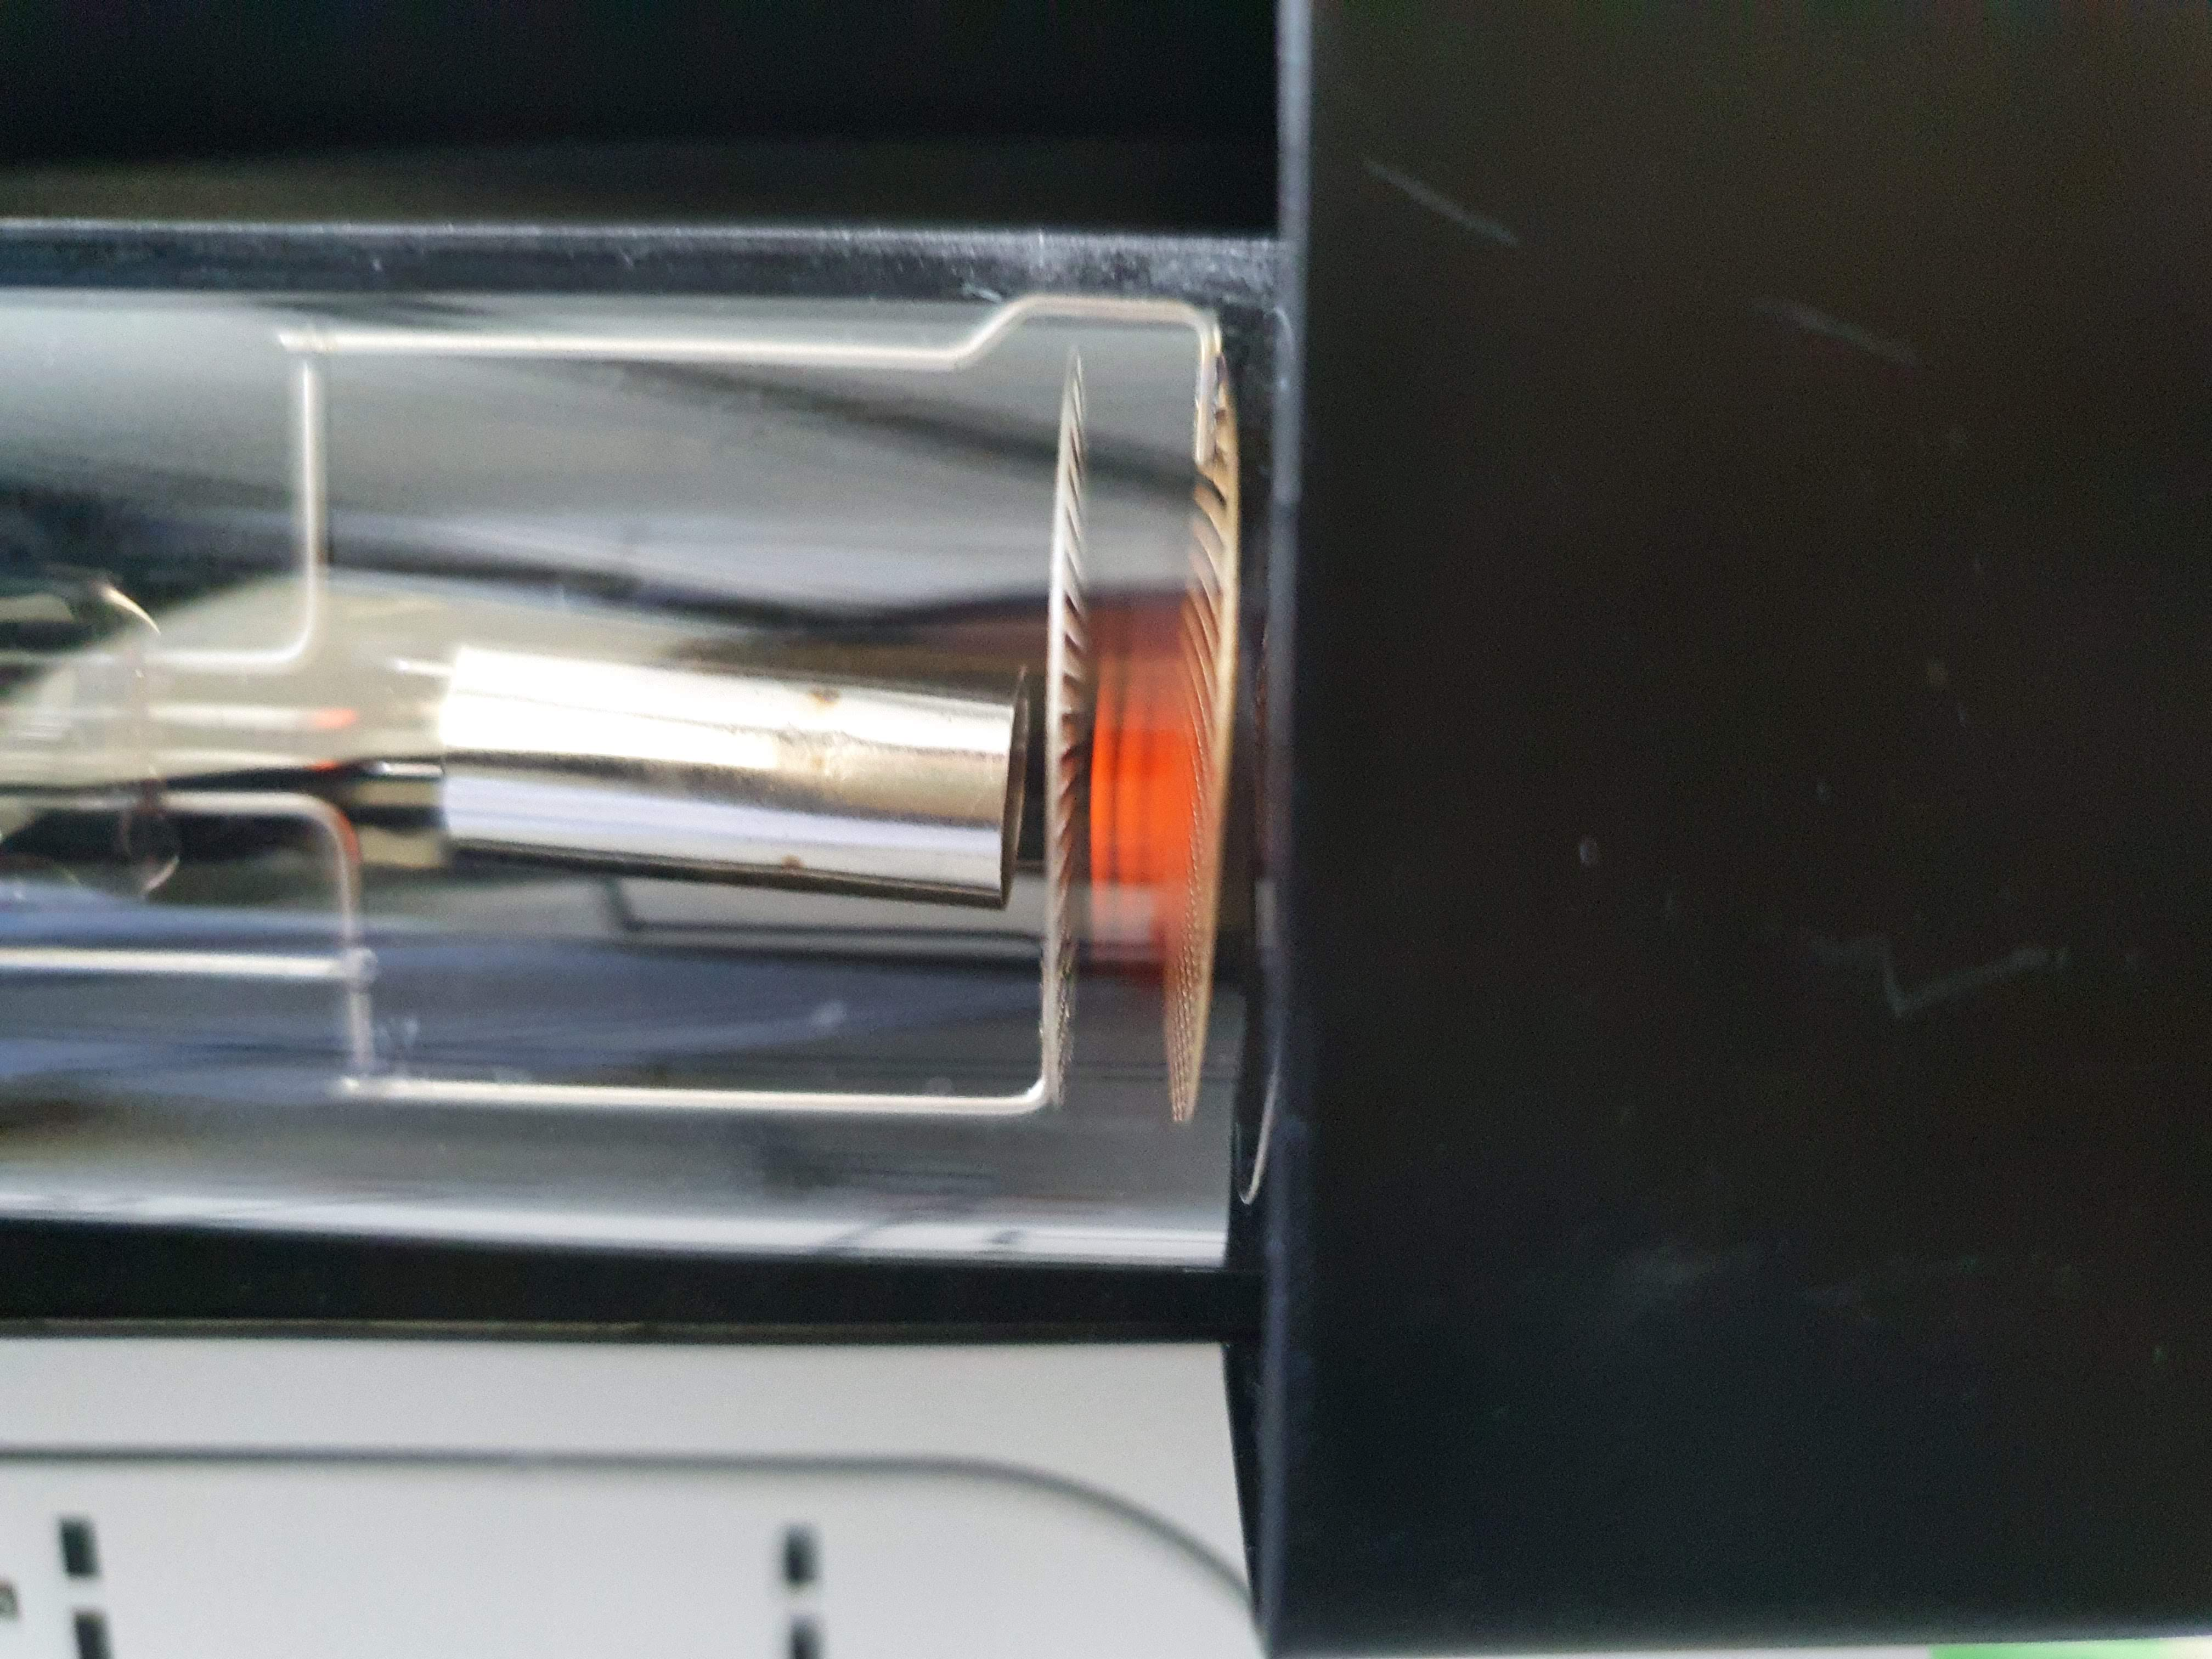
\includegraphics[width=0.6\textwidth]{./images/fhv-neon.jpg}
		    \caption{Die leuchtende Wolken}
		    \label{fig:fhv-neon}
		\end{figure}

		Was mir hier auffällt ist nur die etwa ungewöhnliche $L = \nicefrac{3}{2}$ bzw. $L = \nicefrac{5}{2}$ Zustände. Zu diesem Thema habe ich leider nicht viel im Internet gefunden. Ich würde mich freuen, wenn wir das und der in der Aufgabe genannte Widerspruch im Nachgespräch klären können. 

		Was ein Widerspruch sein könnte ist vielleicht: Mit einem Bohrischen Atommodell stellen wir diskrete Energieniveau vor, es ist also scharfe Minima wie in Teilversuch 1 erwartet. Jedoch sehen wir hier keine scharfe Minima, sondern auch kleine locale Minima innerhalb der etwa größere Minima. (Unterstruktur)

		Ein andere Widerspruch könnte auch sein, dass das Bohrische Atommodell sagt voraus, dass 

	\subsection{Zur Frage 5}
		Die Unterstruktur, die man beim dritten Minima erkennen kann, lässt sich vermütlich mit der Feinstrukturaufspaltung erklären. Wegen 




	